\begin{figure}[t]
  \centering
  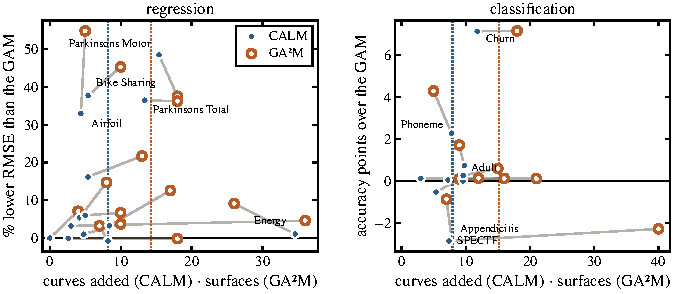
\includegraphics[width=\linewidth]{images/tradeoff}
  \caption{What each model asks a reader to inspect beyond the GAM's one curve per feature, against what it gains over the GAM (24 datasets, Electrical excluded; means over 5 folds).
    For \method{} the count is its splits, each of which adds one curve; for the \gamm{} it is its pairwise surfaces.
    One dot (\method) and one ring (\gamm) per dataset, joined; dotted lines mark the means.
    \method{} inspects 8.2 added curves on average against 14.3 surfaces in regression and 7.9 against 15.2 in classification, and recovers about 60\,\% of the \gamm's gain where that gain exceeds one point.
    Significance is marked in Tables~\ref{tab:clf-acc} and~\ref{tab:regr-rmse}.}
  \label{fig:tradeoff}
\end{figure}
